\startchapter{Object Definitions, Triggers and Event Selection}
\label{chapter:objects}

This chapter describes the physics objects which are reconstructed on an event-by-event basis using collision data from the ATLAS detector and used in this DM search. It also discusses the triggers and event selection cuts which are applied to define the subsets of collision data and MC simulated data, also known as ``analysis regions", which are used for the search. 

\section{Object Definitions}
\label{ap:object_defs}

The goal of the ATLAS detector is to identify particles that are produced by the proton-proton collisions that take place in the centre of the detector, and to reconstruct their kinematic properties. The particle identification and reconstruction is performed using various collections of measured signals in the detector sub-systems, which are broadly referred to as ``physics objects" \cite{physics_objects_atlas_2013}. The physics objects used to reconstruct all particles considered in this search are described in the following sections.

\subsection{Charged Leptons}
\subsubsection{Electrons}
\subsubsection{Muons}
\subsection{Small-radius \aktfour jets}
\subsection{TAR jets}
\subsection{\met}
\subsection{Dark Higgs Candidate Mass}

\begin{itemize}
\item State the trigger combination used for the search (\met OR single muon)
\item Show trigger efficiency curves for \met only and \met OR single muon to show that the (OR single muon) is a necessary addition in the muon channel to achieve 100\% sensitivity.
\item Explain why \met trigger alone is insufficient in the muon channel due the exclusive use of calorimeter information by the ATLAS \met trigger.
\end{itemize}

\section{Event Selections}
\label{sec:evt_selections}

\begin{itemize}
\item High level discussion of why we apply event selections, and goals for optimal signal region definition.
\begin{itemize}
\item Broadly: maximize predicted signal content and minimize simulated background content, while maintaining sufficient MC and data statistics to enable a meaningful comparison between MC and data.
\item Prioritize optimization of signal points near the edge of expected search sensitivity. 
\item Keep signal region blind during optimization to avoid biasing selection.
\end{itemize}
\item Introduce variables used for event selection. Distinguish between variables that are optimized (eg. \mtlepmet) vs. fixed (eg. 1-lepton requirement) during optimization.
\item Present concept and implementation of signal region optimization strategy.
\item High-level discussion of why we define CRs to constrain normalizations of dominant \wjets and \ttbar backgrounds.
\begin{itemize}
\item Provides data-driven normalization constraint which can be extrapolated to the signal region (more details on extrapolation procedure in Chapter 7)
\item Reduces the impact of (and reliance on) theoretical uncertainties involved in simulating the correct normalizations for these backgrounds. Emphasize the difficulty involved with assigning reliable theoretical uncertainties, and hence the value of using data-driven constraints.
\end{itemize}
\item Summary of design goals for control region
\begin{itemize}
\item High purity of background of interest.
\item Orthogonal to SR.
\item Phase space kinematically similar to SR.
\item Signal contamination negligible compared with uncertainty of total background yield.
\end{itemize}
\item Present the \wjets control region, and motivate the \dR reversal used to define it.
\item Present the \ttbar control region, and motivate the \bjet veto reversal used to define it.
\item Present the additional modifications that were needed in the \merged category to optimize the CR definitions
\begin{itemize}
\item Reducing the lower bound on \metsig to boost stats.
\item Increasing the lower bound on \dR in the \wjets CR to reduce the signal contamination to an acceptable level.
\end{itemize}
\item Summary of all analysis regions.
\end{itemize}

\section{Triggers}
\label{sec:triggers_evt_selection}

As described in Section \ref{sec:trigger}, the ATLAS trigger system only saves collision events during data collection which pass both the hardware-based level-1 (L1) trigger and the software-based high-level trigger (HLT). The L1 trigger and the HLT are each comprised of numerous sets of selection criteria, which are also referred to as triggers. Any collision event which satisfies at least one of the triggers which comprise the L1 trigger is processed by the HLT, and likewise if the event satisfies any of the triggers which comprise the HLT it will be kept for later analysis.

The search presented in this thesis is interested in events which produce a single energetic lepton due to the \(s\rightarrow WW(q\bar{q}\ell\nu)\) decay, in addition to high \met due to both the undetected boosted DM in the final state and the undetected \(\nu\) from the \(W\rightarrow \ell\nu\) decay. It is important to determine the efficiency with which the ATLAS trigger system accepts events in the region of phase space defined by the event selections described in Section \ref{sec:evt_selections} above. The efficiency quantifies the probability that an event that the triggers are designed to accept successfully passes the trigger criteria and gets accepted. If the trigger efficiency is \(<100\%\) in any area of the phase space considered in the analysis, it is in general necessary to apply scale factors to any MC simulated events which fall into this phase space to account for the fact some events would have been rejected by the trigger during actual data-taking. It is also then necessary to evaluate and propagate uncertainties associated with these scale factors.

To simplify the trigger efficiency analysis and determine whether any scale factors may be needed, it is helpful to identify a minimal list of triggers which all events considered in the analysis would be expected to pass. One of the event selection criteria for the analysis, presented in Section \ref{sec:evt_selections}, requires all events to have \(\met > 200 \GeV\). Since the ATLAS \met trigger, described in Refs. \cite{met_trigger_performance_2020} and \cite{met_performance_2019}, is designed to efficiently select events with \(\met>150~\GeV\), it is reasonable to expect events which pass the event selection criteria to have also passed the \met trigger with a high efficiency. The specific \met triggers in the ATLAS trigger menu which are considered in this study are chosen following ATLAS recommendations, and vary between different data collection periods defined by ATLAS. The full list of \met triggers used, along with the associated data collection period for each, is listed in Table \ref{tab:summary_triggers_used}.

\begin{table}[ht]
\caption{Summary table of \met triggers from the ATLAS trigger menu used for the search, along with the associated data collection period for each trigger.}
\label{tab:summary_triggers_used}
\footnotesize{
	\begin{center}
	\begin{tabular}{l l }
		\toprule
			Period & MET Trigger \\
			\midrule
			\midrule
			2015 & \textsc{HLT\_xe70\_mht} \\
			\midrule
			2016 (A-D3) & \textsc{HLT\_xe90\_mht\_L1XE50} \\
			\midrule
			2016 (D4-F1) & \textsc{HLT\_xe100\_mht\_L1XE50} \\
			\midrule
			2016 (F2-) & \textsc{HLT\_xe110\_mht\_L1XE50} \\
			\midrule
			2017 (B-D5) & \textsc{HLT\_xe110\_pufit\_L1XE55} \\
			\midrule
			2017 (D6-K) & \textsc{HLT\_xe110\_pufit\_L1XE50} \\
			\midrule
			2018 (B-C5) & \textsc{HLT\_xe110\_pufit\_xe70\_L1XE50} \\
			\midrule
			2018 (C5-) & \textsc{HLT\_xe110\_pufit\_xe65\_L1XE50} \\
		\bottomrule
	\end{tabular}
	\end{center}
	}
\end{table}

The ATLAS trigger system also includes single-muon and single-electron triggers, which are designed to pass events in which a single muon (electron) is reconstructed in the final state which satisfies some minimum \pt requirement. Since the final state considered in the search requires a single charged lepton in the final state, events passing the event selection would also be expected to pass these charged lepton triggers with high efficiency. The specific single muon and electron triggers considered in this study, along with the ATLAS data-taking period(s) in which they were applied, along with the minimum lepton \pt requirement associated with each trigger, are listed in Tables \ref{tab:summary_muon_triggers_used} and \ref{tab:summary_electron_triggers_used}, respectively.

\begin{table}[ht]
\caption{Summary table of single muon triggers from the ATLAS trigger menu used for the search, along with the associated data collection period for each trigger. The minimum muon \pt threshold of each trigger is also listed.}
\label{tab:summary_muon_triggers_used}
\footnotesize{
	\begin{center}
	\begin{tabular}{l l l }
		\toprule
			Periods & Single Muon Trigger & Muon \pt threshold \\
			\midrule
			\midrule
			2015 & \textsc{HLT\_mu20\_iloose\_L1MU15} & 20 \GeV \\
			\midrule
			2016 (A, B-D3, D4-E, F-G2, G3-I3, I4-), & \multirow{3}{*}{\textsc{HLT\_mu50}} & \multirow{3}{*}{50 \GeV} \\
			2017 (B-), & & \\
			2018 & & \\
			\midrule
			2016 & \textsc{HLT\_mu24\_iloose} & 24 \GeV \\
			\midrule
			2015, & \multirow{2}{*}{\textsc{HLT\_mu40}} & \multirow{2}{*}{40 \GeV} \\
			2016 (A) & & \\
			\midrule
			2016 (B-D3, D4-E) & \textsc{HLT\_mu24\_ivarmedium} & 24 \GeV \\
			\midrule
			2016 (D4-E, F-G2, G3-I3, I4-),  & \multirow{3}{*}{\textsc{HLT\_mu26\_ivarmedium}} & \multirow{3}{*}{26 \GeV} \\
			2017 (B-), \\
			2018 \\
		\bottomrule
	\end{tabular}
	\end{center}
	}
\end{table}

\begin{table}[ht]
\caption{Summary table of single electron triggers from the ATLAS trigger menu used for the study presented in Section \ref{sec:triggers_evt_selection}, along with the associated data collection period for each trigger. The minimum electron \pt threshold of each trigger is also listed.}
\label{tab:summary_electron_triggers_used}
\footnotesize{
	\begin{center}
	\begin{tabular}{l l l }
		\toprule
			Periods & Single Muon Trigger & Electron \pt threshold \\
			\midrule
			\midrule
			2015 & \textsc{HLT\_e24\_lhmedium\_L1EM20VH} & 24 \GeV \\
			\midrule
			2015 & \textsc{HLT\_e60\_lhmedium} & 60 \GeV \\
			\midrule
			2015 & \textsc{HLT\_e120\_lhloose} & 120 \GeV \\
			\midrule
			2016 (A, B-D3) & \textsc{HLT\_e24\_lhtight\_nod0\_ivarloose} & 24 \GeV \\
			\midrule
			2016 (A, B-D3, D4-F, G-), & \multirow{3}{*}{\textsc{HLT\_e60\_lhmedium\_nod0}} & \multirow{3}{*}{60 \GeV} \\
			2017 (B-), & & \\
			2018 & & \\
			\midrule
			2016 (A, B-D3, D4-F, G-)  & \textsc{HLT\_e60\_medium} & 60 \GeV \\
			\midrule
			2016 (A, B-D3, D4-F, G-),  & \multirow{3}{*}{\textsc{HLT\_e300\_etcut}} & \multirow{3}{*}{300 \GeV} \\
			2017 (B-), & & \\
			2018 \\
			\midrule
			2016 (A, B-D3, D4-F, G-), & \multirow{3}{*}{\textsc{HLT\_e140\_lhloose\_nod0}} & \multirow{3}{*}{140 \GeV} \\
			2017 (B-), & & \\
			2018 & & \\
			\midrule
			2016 (D4-F, G-), & \multirow{3}{*}{\textsc{HLT\_e26\_lhtight\_nod0\_ivarloose}} & \multirow{3}{*}{26 \GeV} \\
			2017 (B-) & & \\
			2018 & & \\
		\bottomrule
	\end{tabular}
	\end{center}
	}
\end{table}

The lepton triggers are known to be \(<100\%\) efficient, but the resulting scale factors and associated systematic uncertainties are in general well calibrated by dedicated measurements performed within the ATLAS collaboration. As a result, the charged lepton triggers are useful as a means of independently quantifying the efficiency of the \met trigger, as will be shown in a moment, but if the \met trigger can be shown to pass selected events with 100\% efficiency then it is desirable to simply require all selected events to have passed the \met trigger in order to avoid any application of scaling factors and evaluation of related uncertainties.

The efficiency of the \met trigger in a given region ``X" is defined equivalently for ATLAS data (``data") and MC simulated events (``MC") relative to the single lepton trigger (defined as the logical OR of the single muon trigger and the single electron trigger):

\begin{equation}
\label{eq:met_trig_eff}
\begin{footnotesize}
\text{eff}_\text{\met, region X} = \frac{\sum_i w_i\text{ passing (\met triggers)\&(single lepton triggers)\&(selection cuts for region X)}}{\sum_i w_i\text{ passing (single lepton triggers)\&(selection cuts for region X)}}
\end{footnotesize}
\end{equation}

\noindent where $w_i$ is the total event weight for event \(i\) ($w_i=1$ in the case of data). See Section \ref{sec:evt_wts} for a detailed discussion of weights that are assigned to the MC simulated events. Correction scale factors, dependent on the \pt and \(\eta\) of the final-state lepton in each event, are included in the MC event weights in Eq. \ref{eq:met_trig_eff} to account for the \(<100\%\) trigger efficiency of the single lepton triggers. 

Figure \ref{fig:mettrig} compares the \met trigger efficiency defined in Eq. \ref{eq:met_trig_eff} for MC simulated events and ATLAS data for the region defined with the baseline selections, with the following modifications:

\begin{itemize}
\item The \metsig cut is loosened to \(\metsig>5\) and the \mtlepmet cut is loosened to \(\mtlepmet > 100~\GeV\) to enhance statistics.
\item A range of lower bounds on the \met are considered, from \(\sim100~\GeV\) to \(\sim500~\GeV\).
\item The single charged lepton is required to be an electron (a.k.a. the ``electron channel") in Figure \ref{fig:mettrig_e} and a muon (a.k.a. the ``muon channel") in Figure \ref{fig:mettrig_mu}.
\end{itemize}

\begin{figure}[htbp]
  \centering
     \begin{subfigure}{0.49\textwidth}
     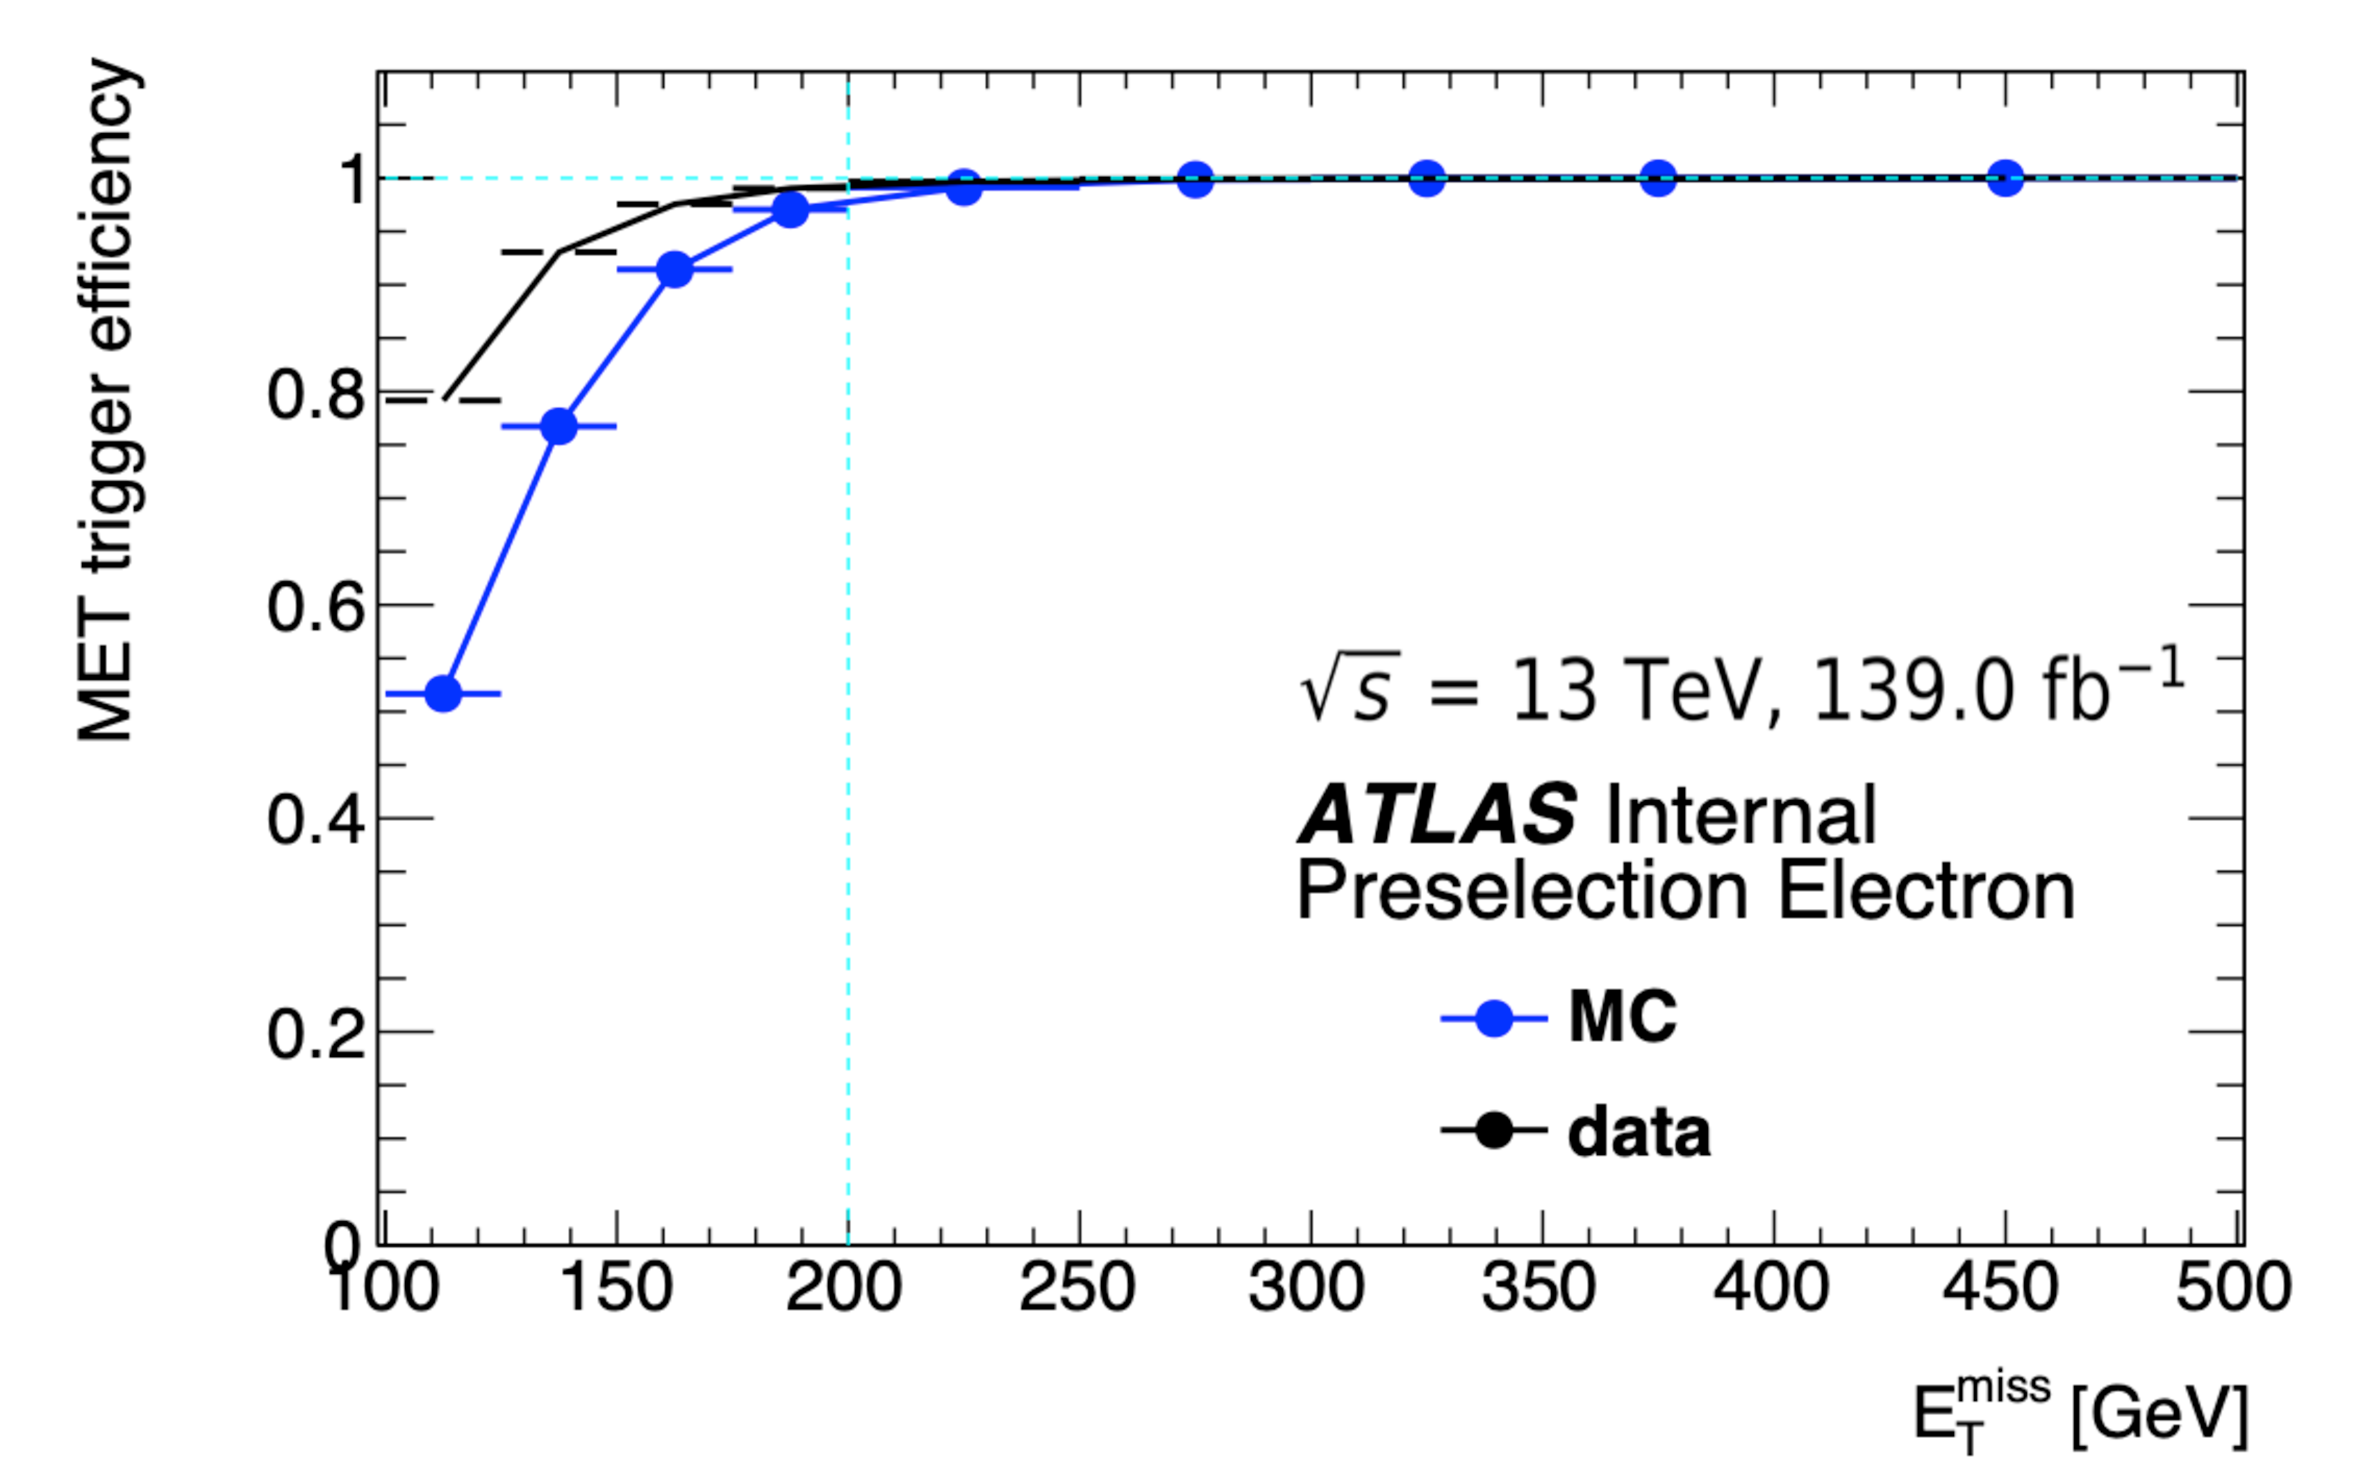
\includegraphics[width = 0.98\textwidth]{Figures/5/PreE_MetTST_met.pdf}
    \caption{Electron Channel}
    \label{ig:mettrig_e}
     \end{subfigure}
    \begin{subfigure}{0.49\textwidth}
     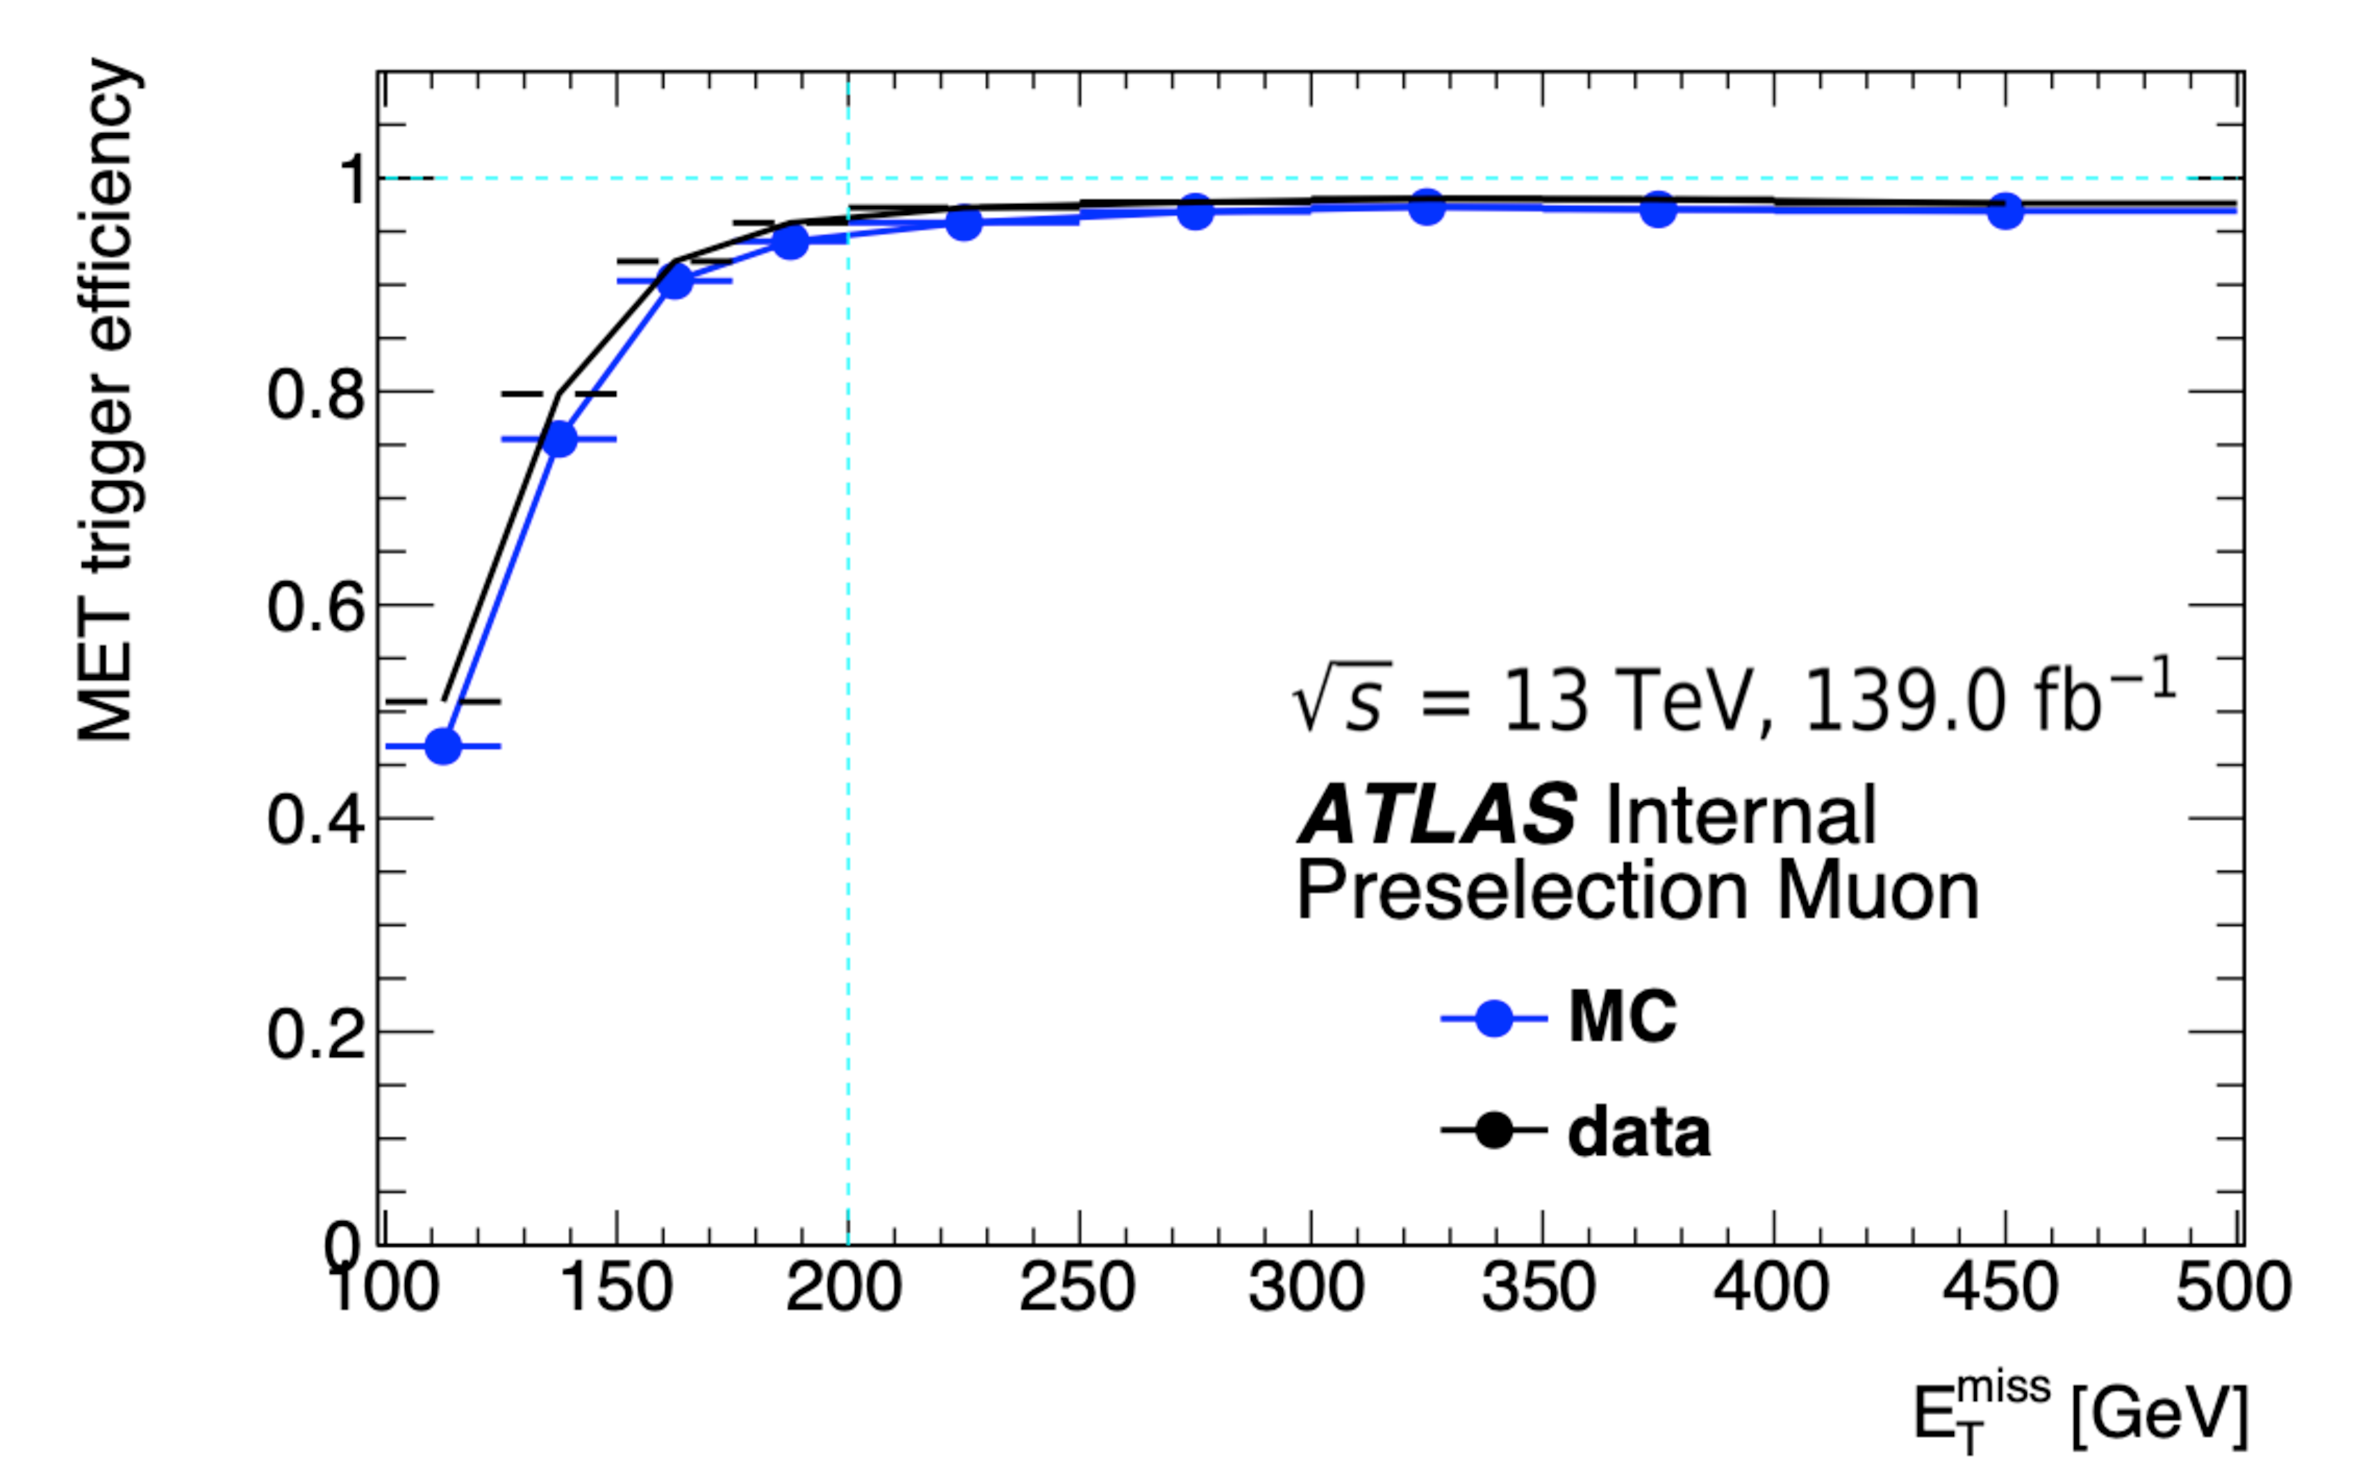
\includegraphics[width = 0.98\textwidth]{Figures/5/PreM_MetTST_met.pdf}
     \caption{Muon Channel}
     \label{ig:mettrig_mu}
     \end{subfigure}
     \caption{Comparison of the \met trigger efficiency defined in Eq. \ref{eq:met_trig_eff}, as a function of the \met lower bound in the event selection, between MC simulated events and ATLAS data in a region defined by a loosened baseline selection. The event selection is separated into electron (left) and muon (right) channels.}
     \label{fig:mettrig}
  \end{figure}
  
Comparing the trigger efficiencies in the Figures \ref{fig:mettrig_e} and \ref{fig:mettrig_mu}, the efficiency in the electron channel converged to 100\% for \(\met > 200~\GeV\), but in the muon channel it instead converges to \(\sim90\%\) for \(\met > 200~\GeV\). After some investigation, the inefficiency in the muon channel was found to be due to events which have large \met arising from high-\pt muons. This is because high-\pt muons largely pass through the ATLAS calorimeter and are detected instead by the muon spectrometer. As a result, such high-\pt muon events can be missed by the \met triggers, which don't make use of information from the muon spectrometer \cite{met_performance_2019}. This can be seen by plotting the \met trigger efficiency using a calculation of \met in the event selection that ignores the muon \pt (a.k.a. ``muon invisible") in Figure \ref{fig:metmuinvis}, and observing that in this case the efficiency converges to 100\% for \met (muon invisible) > 200~\GeV. These high-\pt muon events can, however, be recovered by additionally accepting events which pass the single muon trigger.

\begin{figure}[htbp]
    \centering
     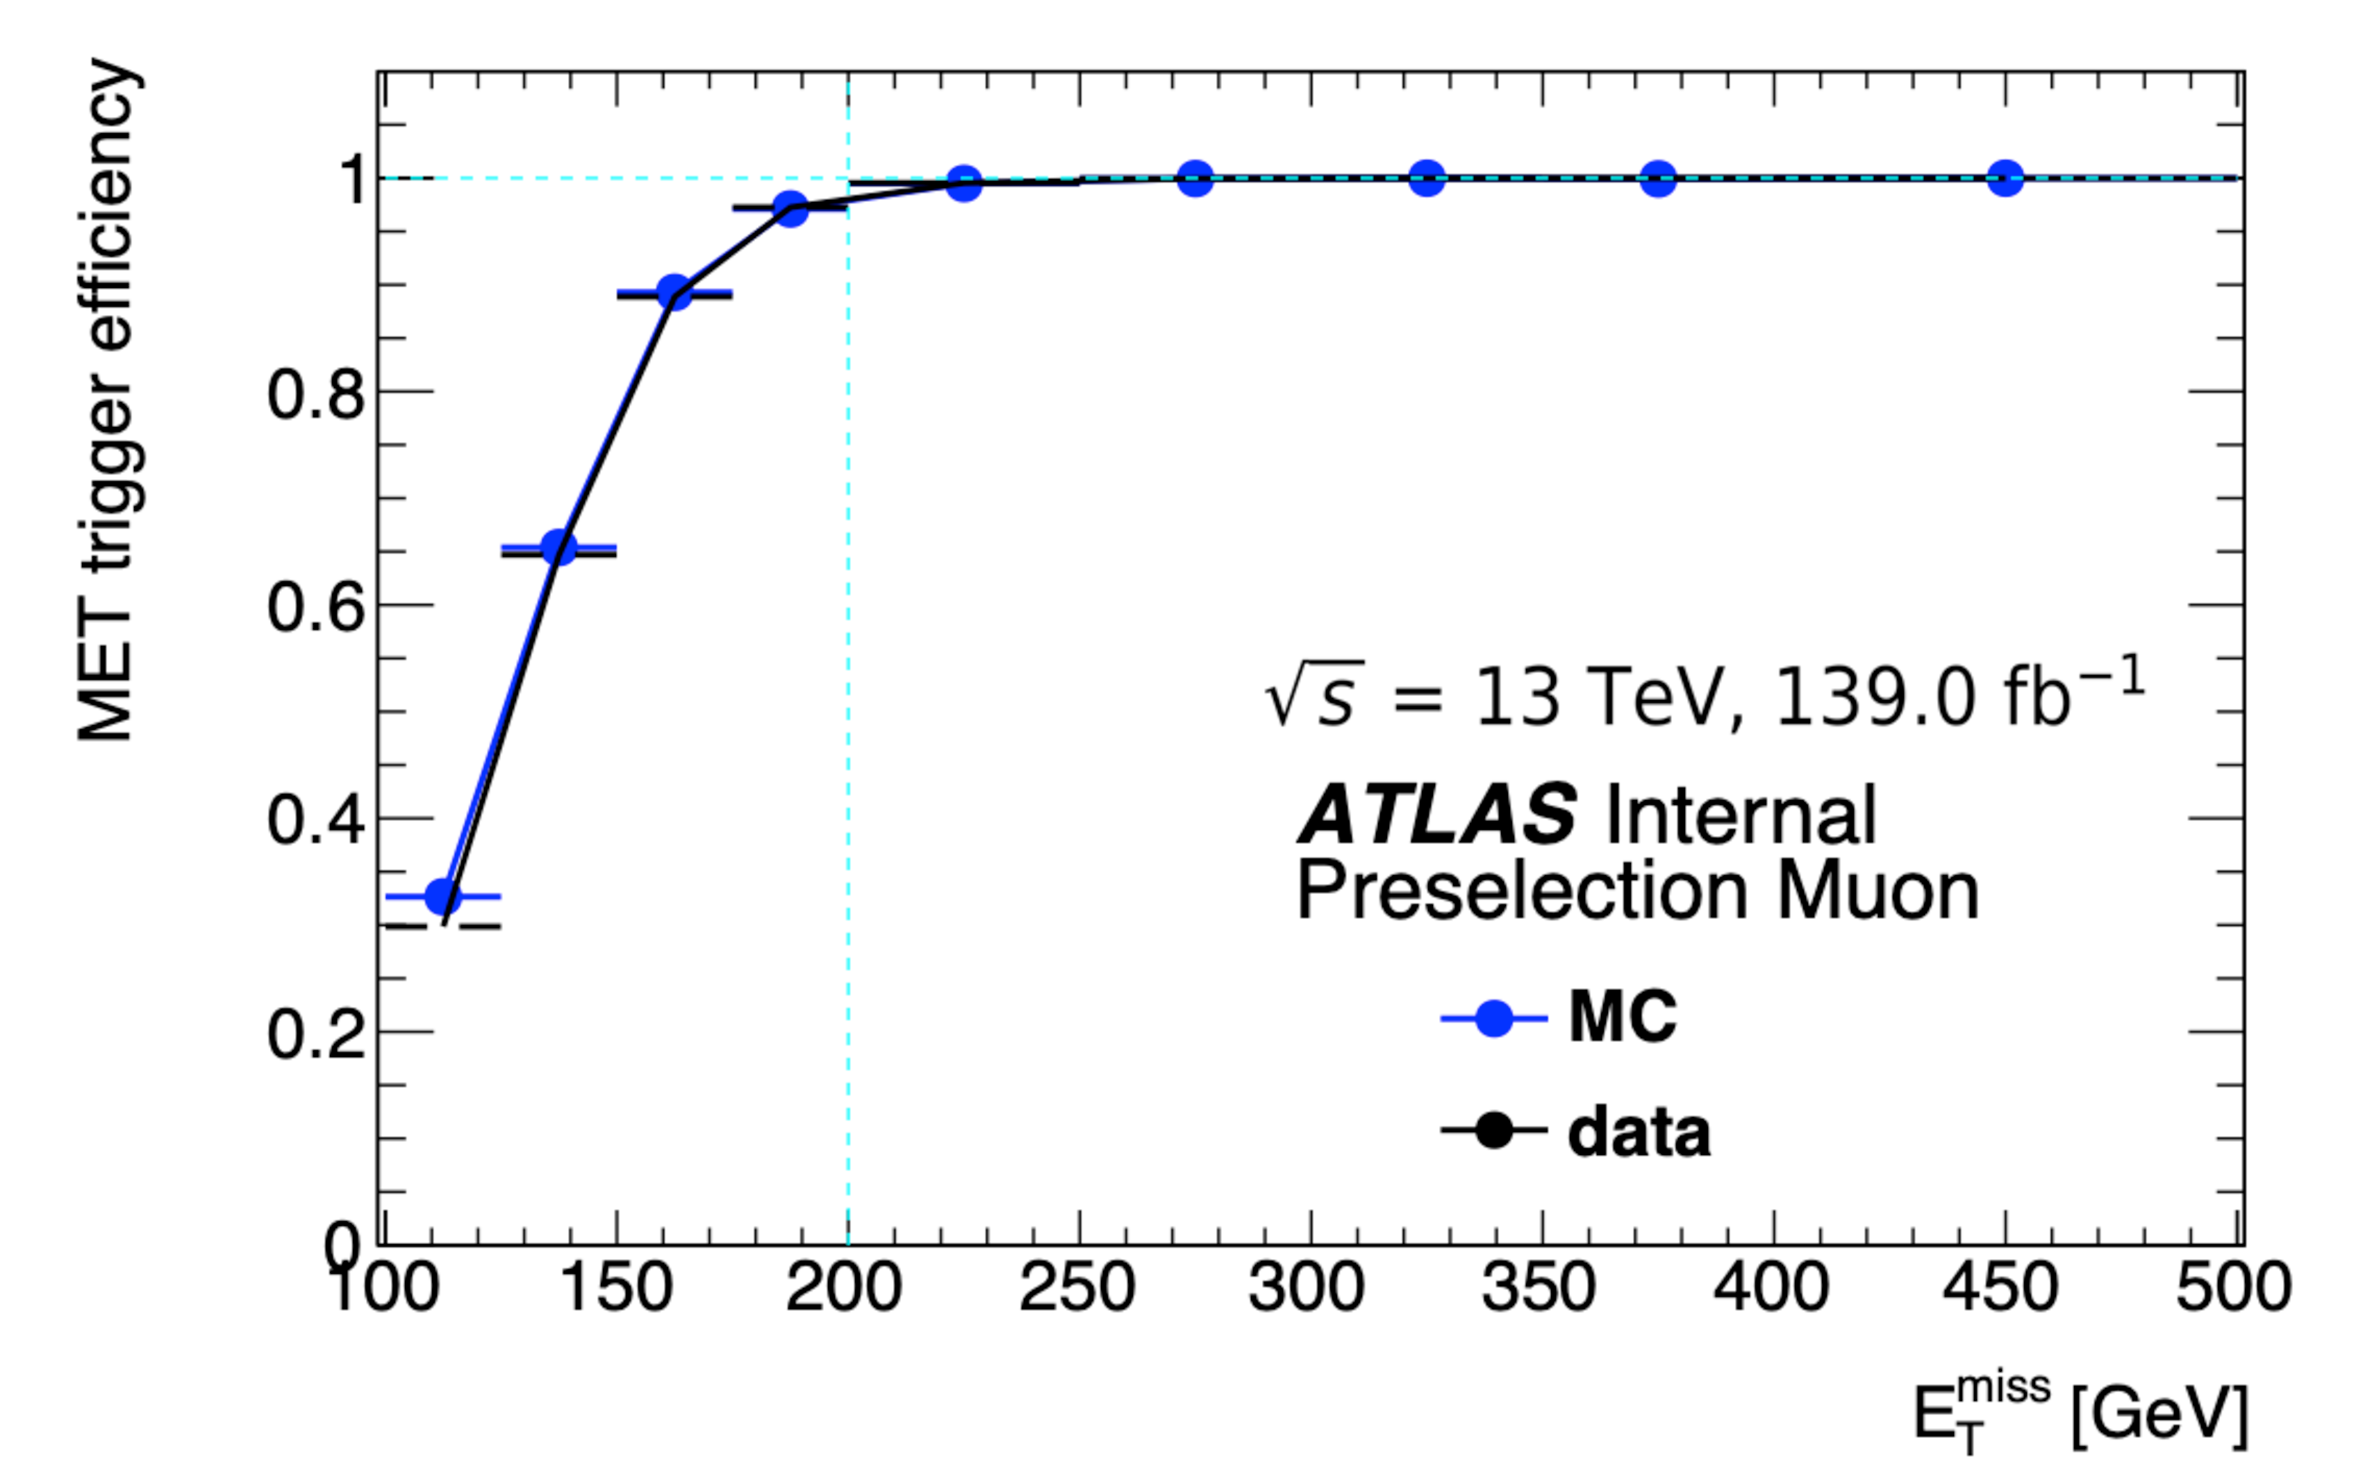
\includegraphics[width = 0.6\textwidth]{Figures/5/Pre_MetTST_met.pdf}
     \caption{\met trigger efficiency, as a function of the \met lower bound in the event selection for the baseline selection in the muon channel, with muons treated as invisible in the calculation of \met}
     \label{fig:metmuinvis}
  \end{figure}

In order to be considered for this search, events are required to have passed either the high-\met trigger (also referred to simply as the ``\met trigger), or the single muon trigger.
